% !TeX spellcheck = en_US

\chapter{The On-board Software Reference Architecture (OSRA)}
\label{chap:OSRA}
\section{Introduction}
\subsection{Background}
Space industry has recognized for the past decade the need to raise the level of standardization in the avionics system in order to increase the efficiency and reduce cost and schedule in the development \cite{SAVOIR}.
The implementation of such a vision is expected to provide benefits for all the stake-holders in the space community \cite{SAVOIR}:

\begin{description}
\item  [Customer Agencies] Significant reduction in the project development cost and schedule and the risk involved in software development.
\item [System Integrators] Increased competition among stake-holders to deliver at lower price and maintain shorter time-to-market as a result of multi-supplier option.
\item [Supplier Industry] Benefits from diversified customer bases and the supplied building blocks would be compatible with software architectures from the software primes such as Thales Alenia Space and Astrium Satellites (EADS Astrium).
\end{description}

Similar initiatives have already been taken across various industries and eg., \ac{autosar} for the automotive industry is worthy mentioning \cite{BasConAUTOSAR}. Space can benefit from these examples, by studies related to how these or similar initiatives were successfully conducted and how they faired. Although the business model is different in the automotive and the space sectors, AUTOSAR demonstrates that the need for standardization is the key irrespective of sectors and is actually driven by the need of the industry to become more competitive \cite{EfAnAUTOSAR}.

Space primes and on-board software companies have made significant progress and have implemented and/or are implementing principle of reuse on the basis of their internal software reference architectures and building blocks. However, for this standardization to provide maximum benefits, it has to be tackled at the European level rather than at a company level \cite{SAVOIR}.

\ac{esa} through its two parallel activities, namely \ac{cordet} and \ac{domeng} \cite{CORDET}, which aimed at increasing the software reuse in on-board software have confirmed that interface standardization allows to efficiently compose the software on the basis of existing and mature building blocks.

To refer to all the ongoing initiatives and to provide a platform for technical discussions related to the vision of avionics development through maximizing reuse and standardization, a \ac{savoir} Advisory Group (SAVOIR Advisory Group) was created. SAVOIR Advisory Group decided to spawn a specific subgroup for on-board software reference architectures called SAVOIR Fair Architecture and Interface Reference Elaboration (SAVOIR FAIRE) working group. \ac{osra} is the result of the R\&D activities of this group \cite{SAVOIR}.   

The OSRA is designed to be a single, common and agreed framework for the definition of the \ac{obsw} of the future European Space Agency (ESA) missions \cite{SAVOIR}. It is based on solid scientific foundations and accompanied by development methodology and architectural practices that fit the domain. A single software system would thus be an "instantiation" of the reference architecture to specific mission needs \cite{PhdThesis}\cite{SAVOIR}.

\section{Need for software reference architecture}
\subsection{Motivation}
According to the ISO/IEC standard ISO 42010 \cite{ISO42010}, the software architecture is defined as: 

\textit{"The fundamental organization of a system embodied in its components, their relationships
to each other, and to the environment, and the principles guiding its design and evolution"}
 
A software architecture is the key to create "good quality" software because it promotes architectural best practices and contributes to the quality of the software. A bad architecture hinders the fulfillment of functional, behavioral, non-functional and life-cycle requirements \cite{PhdThesis}.

According to the "\ac{rup}" \cite{RUP}, the software reference architecture can be defined as:

\textit{"A predefined architectural pattern, or set of patterns, possibly partially or
completely instantiated, designed, and proven for use in particular business and technical contexts, together with supporting artifacts to enable their use. Often, these artifacts are harvested
from previous projects"} 

A software reference architecture prescribes the form of concrete software architectures for a set of systems for which it is developed. So, a reference architecture is a form of "generic" software architecture which prescribes the founding principles, the underlying methodology and the architectural practices that are recognized by the domain stakeholders as the best solution to the construction of a certain class of software systems  \cite{PhdThesis}\cite{SoftRefArch}.

Elevating a software architecture to a software reference architecture permits to gather and re-use lessons learned and architectural best practices, give new projects a consolidated running start and promote a product line approach \cite{SAVOIR}.

A generic software reference architecture is made up of two main parts \cite{SAVOIR}:

\begin{description}
\item [Software architectural concepts] These address the pure software architectural related issues.
\item [Architectural building blocks and interfaces] These are related to functional aspects and the corresponding interface definitions which express functions derived from the analysis of the functional chains of the core on-board software domain. 
\end{description}

\begin{figure}[h]
	\centering
	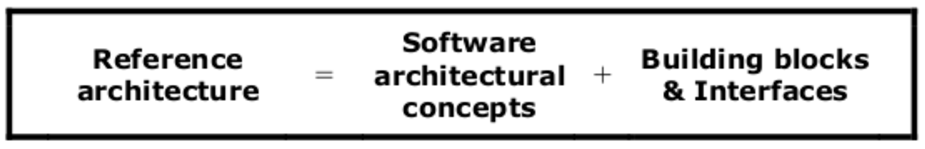
\includegraphics[width=0.8\textwidth]{SoftwareReferenceArchitecture.pdf}
	\caption{Parts of a software reference architecture}
	\source{\cite{SAVOIR}}
	\label{}
\end{figure} 

As mentioned in the previous section, in order to increase the efficiency and cost-effectiveness in the development process of on-board avionics and to incorporate more number of functionalities in the on-board software, the overall objective of space industry would be to standardize the avionics systems and therefore the on-board software.

A building block approach is one of the ways to tackle this problem. In this approach, the on-board software is implemented from a set of pre-developed and compatible building blocks, plus specific adaptations and "missionisation" according to specific mission requirements \cite{SAVOIR}. The target missions are the core ESA missions, i.e. high reliability and availability spacecraft driven systems (eg. operational missions, science missions).

The "right" building blocks need to be produced and supplied by the suppliers to any system integrator and to achieve this, reference architectures need to be defined.

A software building block, generally \cite{SAVOIR}:
\begin{itemize}
\item Has a clear, well defined, specified, documented function and open external interfaces for the purpose of interaction.
\item Meets defined performance, operation and other requirements.
\item Is self-contained so that they can be used at higher-integration levels eg. board, equipment, subsystem. 
\item Has a quality level that can be assessed.
\item Is applicable in well defined physical and hardware environment.
\item Is worth developing as they are going to be used in bulk of ESA missions.
\item Is designed for reuse in different projects, by different users under different environments.
\item Can be made available off-the-shelf, ready for deployment under different conditions.  
\end{itemize}

Separation of the application aspects from the general-purpose data processing aspects is the key to generic/reusable software architectures \cite{PhdThesis}. The lower layers of the architectures usually handle the implementation of communication, real time capabilities etc. and the higher level layers usually deal with the application aspects. However there have to be ways to annotate the application building blocks (ABB) with sufficient information regarding requirements related to communication, real-time, dependability etc., so that the platform building blocks (PBB) can provide a suitable complete implementation. Development of interface specifications with reference architectures as a basis, allows the implementation of the famous AUTOSAR concept: \textit{"Cooperate on standards, compete on implementation"}\cite{AUTOSARurl}.

The OBSW life-cycle needs to be consistent with the system life-cycle, which features the definition of functional increments in system development \cite{SAVOIR}. Hence, OBSW must in particular:

\begin{itemize}
\item Allow for faster software development.
\item Be compatible to a late definition or changes of some of its requirements.
\item Cope with various system integration strategies.
\end{itemize}

\subsection{User needs}

The COrDeT study, with the slogan "Faster, Later, Software", represented a summary of the above programmatic stakes for the on-board-software life-cycle \cite{CORDET}\cite{SAVOIR}. These stakes are included and defined as the user needs \cite{SAVOIR}\cite{PhdThesis} for the development of OSRA:

\begin{description}
\item [Shorter software development time] Need for faster software development in the context of a shorter schedule. The \cref{fig:RedSWSched} depicts the reduction in the schedule for software development in the future projects. 

\begin{figure}[h]
	\centering
	\includegraphics[width=0.8\textwidth]{ReductionSWSchedule.pdf}
	\caption{Reduction in the schedule for software development}
	\source{\cite{SAVOIR}}
	\label{fig:RedSWSched}
\end{figure}

\item [Reduce recurring costs] Identification and reduction of recurring costs by providing the same set of functions eg., device drivers, real-time operating systems, communication services, etc.   

\item [Quality of the product] Need for high quality software (timing predictability, dependability, etc.) and the quality must be at least the same as one of OBSW developed with current approaches.

\item [Increase cost-efficiency] Increase in the "value" of the software product that is developed for a given amount of budget.

\item [Reduce Verification and Validation effort] The new development approaches shall foster the reduction of effort for \ac{vandv}, which is one of the main contributor to the cost of software development.

\item [Mitigate the impact of late requirement definition or change] 

\item [Support for various system integration strategies] It should be possible to do preliminary software releases which allow early system integration efforts.

\item [Simplification and harmonization of FDIR] A simplification and hopefully, harmonization of the \ac{fdir} approach is advocated.

\item [Optimize flight maintenance] There should be provision for changing the OBSW during flight maintenance and coordination of strategies to perform it. 

\item [Industrial policy support] Enable multi-team software development, so that sub-contracting to the non-primes is possible, while still being in-charge of the integration.

\item [Role of software suppliers] Increase competence of supplier and foster competition among them. 

\item [Dissemination activities] System engineers should be exposed to the core principles of the process.

\item [Future needs] Future needs such as integration of functions of different criticality and security levels, use of Time and Space Partitioning (TSP), support to multi-core processors, need to be subjected to evaluation and their impact on software reference architecture need to be monitored.
\end{description} 

\subsection{High level requirements}
\label{subsection: High level requirements}
The user needs are translated into a set of high-level requirements for OSRA \cite{SAVOIR}\cite{PhdThesis}.

\begin{description}
\item [Software reuse] The architecture shall be designed in such a way that the reuse of the functional aspects should be independent of the reuse of the non-functional aspects, reuse of the unit, integration and validation tests are made possible.
 
\item [Separation of concerns] Separation of concerns is one of the cornerstone principles of OSRA and it deals with separating different aspects of the software design, in particular the functional and non-functional concerns. Separation of concerns helps to reuse functional concerns independently from non-functional concerns, which increases the software reuse.
 
\item [Reuse of V\&V tests] The chosen architectural approach should also promote the reuse of Verification and Validation tests that were performed on the software and not just the software itself. The aim is to maximize the reuse of the tests written for the functional part of the component software.

\item [HW/SW Independence] Software should be developed independent from the hardware features. It is necessary to separate parts of the software that interact directly with the hardware, into separate modules and make them accessible through defined interfaces. In this way, as long as the interface does not change, the software is isolated from the changes in the hardware-dependent layers.
	  	
\item [Component based approach] The whole software should be designed as a composition of components that are reusable in nature. The architecture shall respect preservation of properties of individual building blocks, once they are integrated into the architecture and it should be possible to calculate the system's property as a function of components' individual properties. The former is called composability and the latter is called compositionality \cite{CompBasedDev}. \cref{section: Founding principle-Composition} in \cref{chap: Software development process} explains this approach in more detail.
  
\item [Software observability] The software architecture should provide means to observe the software specific parts and extract current and past status of the software using the services specified by its operational scenarios.

\item [Software analysability] The design process and methodology used for the reference architecture shall support the verification of functional and non-functional properties at design time.

\item [Property preservation] The non-functional properties should be considered as constraints on the system as they specify the "frame" in which the system is expected to behave. 
These properties have to be preserved or enforced so that these properties are not only used for the analysis of the software model, but also find their way through to the final system at run-time. Adequate mechanisms should be provided to handle the enforcement of the properties and also mechanisms to handle reactions to violation of these properties. 

\item [Integration of software building blocks] The architecture should allow the combination of coherent building blocks.

\item [Support for variability factors] The architecture shall include design features allowing isolating the variability foreseen in the domain of reuse.

\item [Late incorporation of modification in the software] The architecture should be immune to late modification of the software in the software life-cycle. System integration almost always finds some system problems and it is the responsibility of the software to contain these problems and implement new requirements. The architecture to which the software is conformal to, should be able to handle these late modifications in the software.

\item [Provision of mechanisms for FDIR] The requirements for FDIR, are consolidated often late in the life cycle and the software architecture must accommodate for it.

\item [Software update at run-time] The reference architecture should allow update to single software components as well as their bindings without having to reboot the entire on-board computer as it is a risk for the system and reduces the mission availability/up-time.
\end{description}  

\section{The Software Architectural Concept}
\subsection{Fitting Model-Driven Engineering}
\ac{mde} is a novel trend for software development in the space domain, but has been successfully applied to enterprise computing \cite{CompBasedDev}. The validation-intensive real-time high-integrity systems such as on-board software systems make the adoption of the MDE considerably more arduous. Positive experiences on the application of MDE to the design of these kind of systems do exist and it can be found in the '\ac{chess}: space case study' \cite{CompBasedProcess} and the 'ESA: reference Earth Observation case study' \cite{CompBasedProcess}.

In MDE, the principal design artifact is a model, which is an abstract representation of the system under development, which encompasses systems and software architecture. Each model conforms with a metamodel, which describes the syntax of entities that populate the models, as well as their relationships and the constraints in place between them. The metamodel constrains the design space of the MDE infrastructure \cite{Metamodelling}.  

COrDeT (Component Oriented Development Techniques) study aimed at investigating various techniques in fields such as software product line engineering, model driven engineering and component orientation \cite{CORDET}. Based on this study, the concept of overall software reference architecture, in the development of OSRA, is considered to be made up of \cite{SoftRefArch}\cite{SAVOIR}:

\begin{description}
\item [Component Model] A component model is the basis for designing the software as a composition of individually verifiable and reusable software units \cite{ComponentModel}.

\item [Computational Model] A computational model is used to relate to the design entities of the component model, their non-functional needs for concurrency, time and space, to a framework consisting of analysis techniques, in general, to a set of schedulability analysis equations, which help to judge formally, whether the description of the architecture is statically analyzable \cite{ScheduAnaly}.

\item [A Programming Model] A programming model is used to ensure that the implementation of the design entities obey the semantics and the assumptions of the analysis and the attributes used as input to it \cite{CharEvoRAVCodeAr}.

\item [A conforming Execution Platform] An execution platform helps to preserve at run-time, the properties asserted by the static analysis, and is able to react to possible violations of them.  
\end{description}

These become the key ingredients for the very foundation of the MDE design methodology focused on the principle of correctness by construction and property preservation, which are high level requirements respectively. \cref{fig: Constituents of OSRA} gives a pictorial representation of it.

\begin{figure}[h]
	\centering
	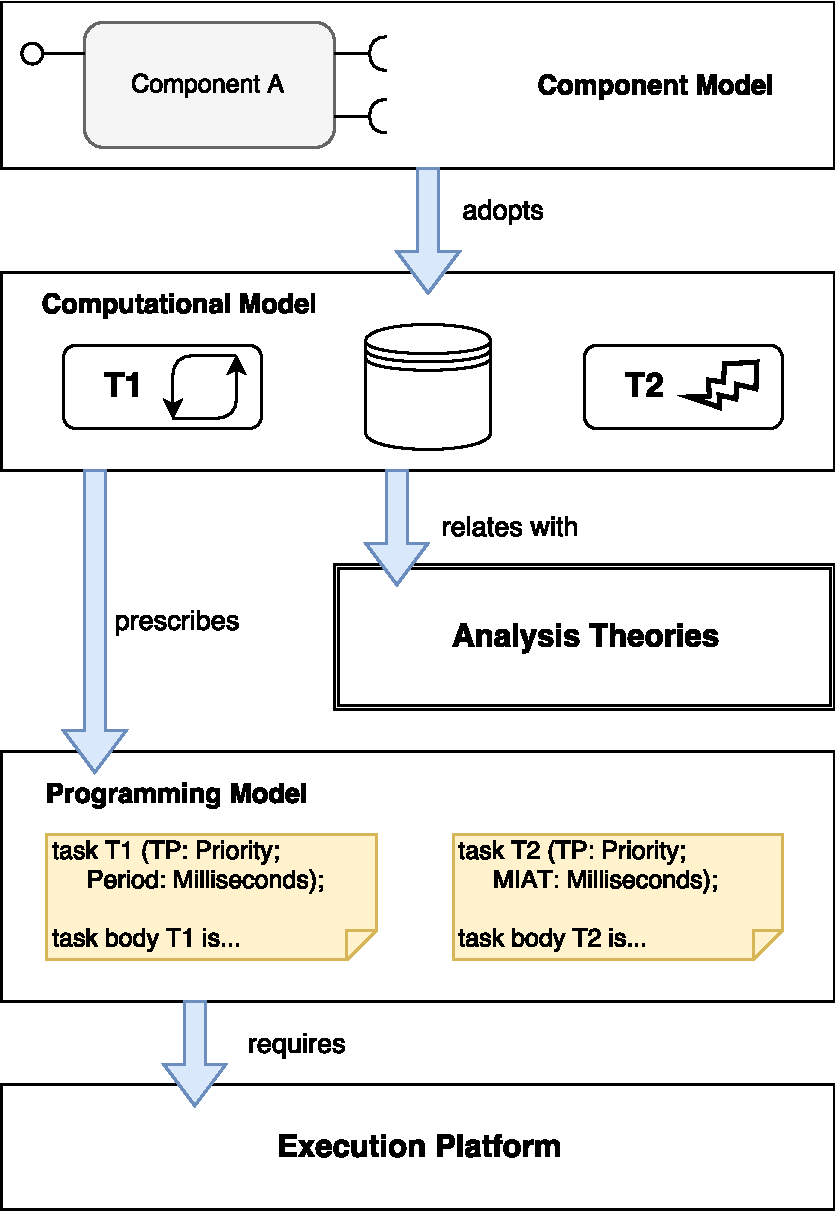
\includegraphics[width=0.5\textwidth]{ConstituentsOfSWArchitecture.pdf}
	\caption{The four constituents of the software reference architecture}
	\source{\cite{PhdThesis}}
	\label{fig: Constituents of OSRA}
\end{figure}

\subsection{Component Model}
\ac{cbse} is a software methodology centered on the systematic re-use of software by realizing the software as an assembly of units of composition called components \cite{CBSE}.
The adoption of Component Based Software Engineering (CBSE) in the context of high-integrity real-time systems in general and in space domain in particular is not so popular as in the other main-stream domains like enterprise computing because of strong verification and validation requirements imposed in the space domain and the presence of non-functional dimensions \cite{SAVOIR}.

The principles of Component Based Software Engineering (CBSE) when combined with the principles below can be used to build OBSW as an assembly of components \cite{SAVOIR}: 
\begin{itemize}
\item Principle of separation of concerns, by allocation of concerns to three distinct software entities: the component (which is a design entity), the container and the connector (which are entities used in implementation only and which do not appear in the design space).
\item Possibility of verification of properties related to composability and compositionality \cite{CompBasedDev}. 
\end{itemize}

The execution platform defined in the software architecture then provides the services to the components, container and the connectors. Finally, the entire software is deployed on the physical architecture (Computational units, equipment, and the network interconnections between them).

\subsubsection{\textbf{Founding principles of choice}}
This section describes the founding principles of choice of the component model:

\begin{description}
\item[Correctness by construction] E.W. Dijkstra in his ACM Turing lecture in 1972 suggested that the program construction should be done after a valid proof of correctness of construction has been developed \cite{CompBasedProcess}. Two decades later, a software development approach called Correctness by Construction (C-by-C) was proposed which advocated the detection and removal of errors at early stages, which led to safer, cheaper and more reliable software \cite{CompBasedProcess}\cite{PhdThesis}. The Correctness by Construction practice follows:
\begin{itemize}
\item To give a solid reasoning on the correctness of the document or code, it is necessary to use formal and precise tools and notations for their development and verification. 
\item Defining things only once so as to avoid contradictions and repetitions.
\item Designing the software that is easy to verify e.g. by using safer language subsets or using appropriate coding styles and software design patterns. 
\end{itemize}

In OSRA and the component model developed along with it, the Correctness by Construction principle is changed to be applicable to a CBSE approach based on Model-driven Engineering (MDE) \cite{CompBasedProcess} wherein:

\begin{itemize}
\item The components can be designed.
\item The products designed by the design environment can be verified and analyzed by the design environment.
\item The lower level artifacts can be automatically generated and the software production can be automated to the maximum extent.  
\end{itemize}

\item [Separation of concerns] 
\label{section: Founding principle-Separation of concerns} 
Separation of concerns was first advocated by Dijkstra \cite{CompBasedProcess} and it helps to separate the aspects of software design and implementation. The OSRA and its associated component model promotes separation of concerns\cite{CompBasedProcess}\cite{PhdThesis}:

\begin{itemize}
\item The components are restricted to hold the functional code only. The non-functional requirements which has effects on the run-time behavior e.g. tasking, synchronization and timing are dealt by the component infrastructure which is external to the component and which realizes the functional code. The component infrastructure mainly consists of containers, connectors and their run-time support.

\item A specific annotation language is specified which is used to define the non-functional requirements and these are annotated on the components realizing the functional code.

By this, model transformations that automatically produce the containers and connectors that serve the non-functional requirements, enable the execution of the schedulability analysis directly on the model of components. This makes the implementation of the non-functional concerns fully compliant with its specification \cite{ScheduAnaly}. 

\item A code generator (whose development is the prime concern of this Master thesis) operates in the back-end of the component model, builds all of the component infrastructure that embeds the user components, their assemblies and the component services that help satisfy the non-functional properties \cite{CharEvoRAVCodeAr}. 
\end{itemize}

\newpage
Inculcating the principle of separation of concerns in the development process has two major benefits \cite{CompBasedProcess}:

\begin{itemize}
\item It increases the reuse potential of the components, which is an important high level requirement described in the previous section \cite{SAVOIR}. The reuse potential of the component is increased because the same component can now be used under different non-functional requirements (as per the instantiations of the component infrastructure).

\item It helps in the generation of vast amount of complex and delicate infrastructural code which takes care of realizing the non-functional requirements at run-time. This increases the readability, traceability and maintainability of the infrastructural code. 
\end{itemize}

\item [Composition] 
\label{section: Founding principle-Composition}
When composability and compositionality can be assured by static analysis, guaranteed through implementation, actively preserved at run-time, the goal of composition with guarantees as discussed by Vardanega can be achieved \cite{CompBasedProcess}. This is also one of the high level requirements defined in the section before.
 
Composability is guaranteed when the properties of individual components are preserved on component composition, on deployment on target and on execution. The components, as mentioned before, implement only the functional code, most part of which is sequential only and they do not have to worry about the non-functional semantics. The components behave like black-boxes and showcase to the external world only the provided and required interfaces. Other components or infrastructural components are expected to communicate through these defined interfaces only. Hence, when components are composed with each other with matching required and provided interfaces, the functional composability is guaranteed which is necessary but not sufficient.

The non-functional requirements/constraints are annotated on the components (specifically the component interfaces) and they are realized by the container which encapsulates the respective component \cite{SAVOIR}\cite{ComponentModel}. The provided interface determines the semantics of the invocation and adds to the functional capabilities provided by the component. These semantics must match with the execution semantics described by the computational model, to which the component model is attached. An example for composable property is shown in \cref{fig: Composability}. In this case, the number of threads and protected objects generated per component, which entirely depends on the extra functional notations to the component interface should be invariant across component composition for the composable property to hold true.  

\begin{figure}[h]
	\centering
	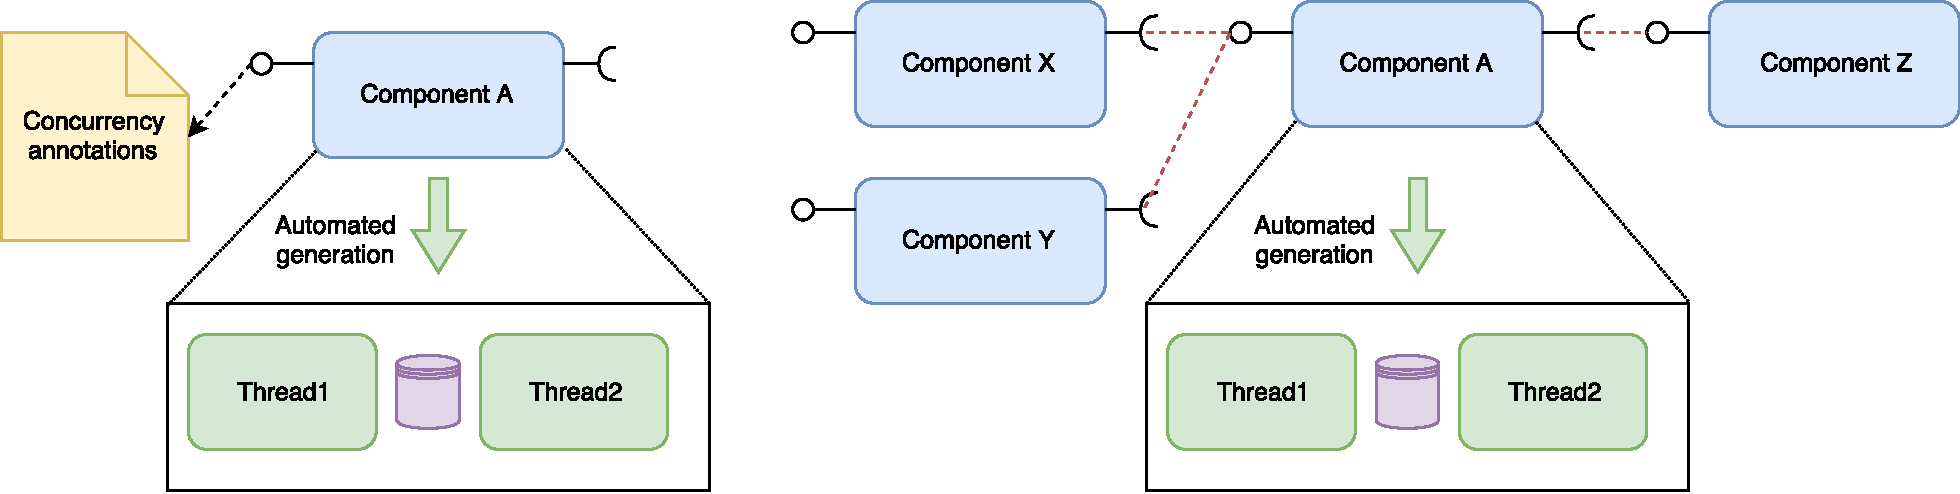
\includegraphics[width=1.0\textwidth]{Composability.pdf}
	\caption{Example for composability}
	\source{\cite{PhdThesis}}
	\label{fig: Composability}
\end{figure}

The computational model chosen should help extend composability to the non-functional constraints e.g. concurrency and the ones related to real-time and make it possible to get a compositional view of how execution occurs at the system level. Compositionality is said to be achieved when the properties of the system as a whole is a function of the properties of the constituting components. Finally, the binding of the computational model to the component should allow the execution semantics of the components with non-functional descriptors to be completely understood. An example for compositionality in shown in \cref{fig: Compositionality}. In this case, it should be possible to calculate the overall latency for the delivery of an output (i.e., the worst-case response time of the end-to-end chain of activities) from individual latencies of different components for the property of compositionality to hold true.

\begin{figure}[h]
	\centering
	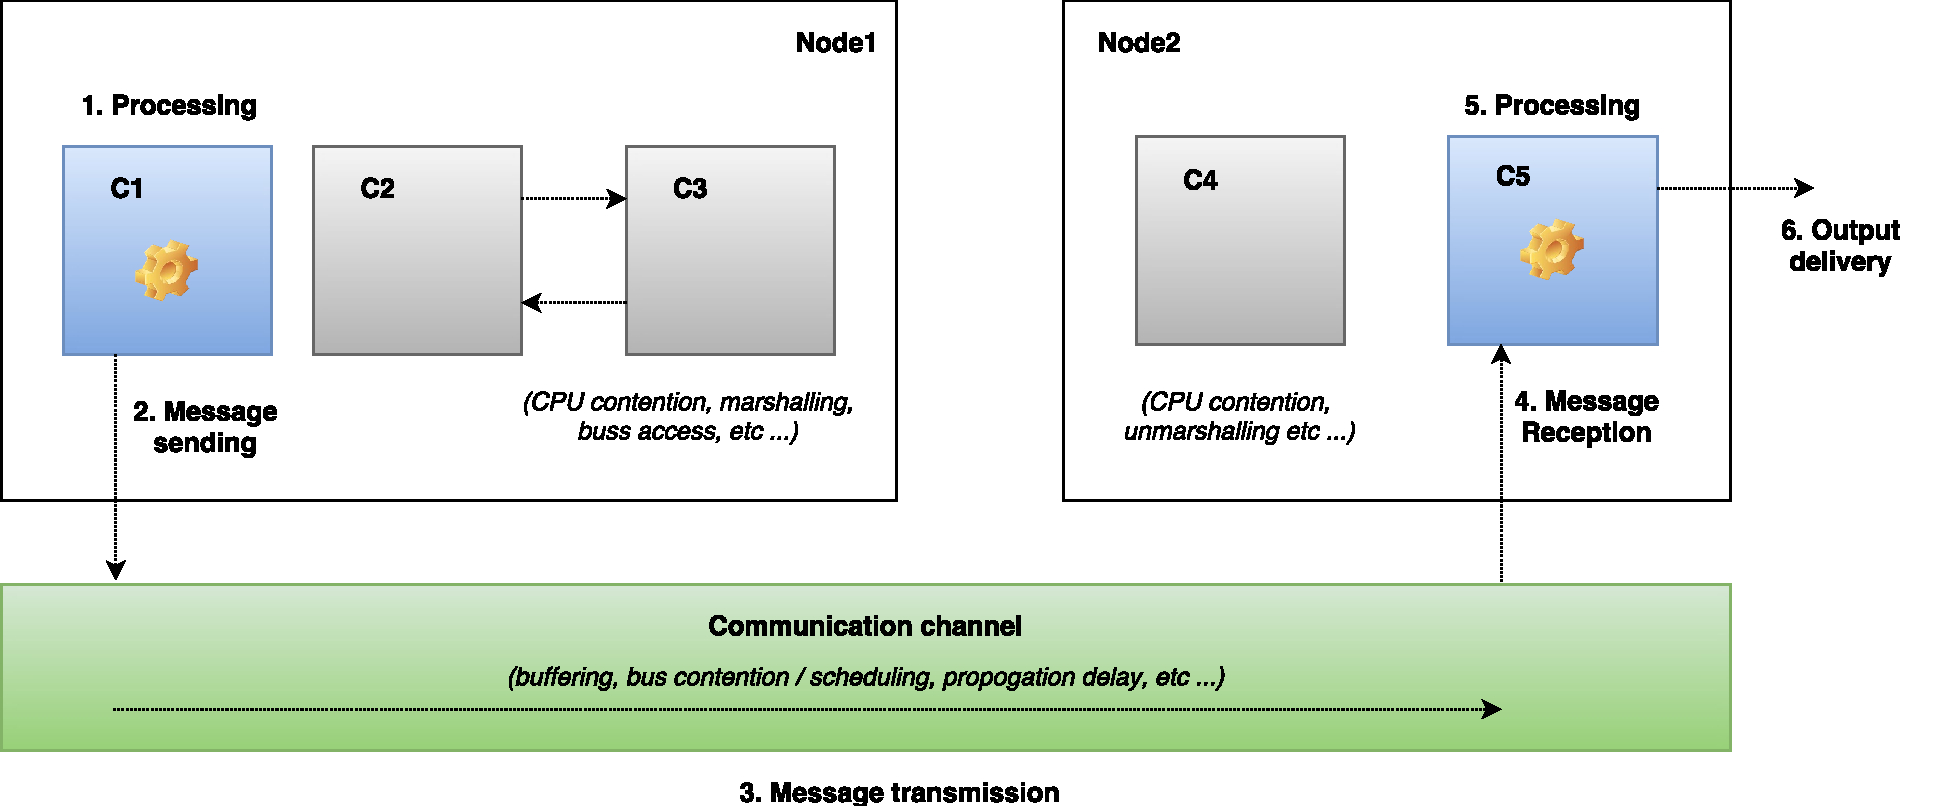
\includegraphics[width=1.0\textwidth]{Compositionality.pdf}
	\caption{Example for compositionality}
	\source{\cite{PhdThesis}}
	\label{fig: Compositionality}
\end{figure} 

In OSRA, the first and second needs can be met by having correct representations of the non-functional attributes in the component interfaces and the third need is taken care of by the generation of proper code artifacts, which is the main concern of this Master thesis.     
\end{description}

\subsubsection{\textbf{Software entities}}
\label {section: Software entities}
The following section describes more about components, containers and the connectors.

\begin{description}
\item[Component] Chaudron and Crnkovic describe that a Component model defines standards for properties that individual components must satisfy and the methods and possibly ways to compose components \cite{CompBasedProcess}.

A component provides a set of services and exposes them to the external world as a "provided interface". The service which is needed from other components or the environment in general are declared in a "required interface". A particular component connects to other components in order to satisfy the needs of its required interfaces. An event based communication system is also possible between components and a component can register to an "event service" to get notified about events emitted by other components.

Non functional attributes are added to the component interfaces as discussed before in the previous section on separation of concerns.

The adoption of hierarchical decomposition of components can be an effective way of defining components instead of defining a containment relationships. A child component can be developed to any component which would delegate and subsume the relationships between the interfaces of the child component and its parent. But the drawback is that various non-functional dimensions applicable to the space domain complicate the picture and hence is hierarchical decomposition of components not allowed at the current stage of development \cite{PhdThesis}.
    
\item [Container] The container is a software entity that wraps around the component, which is directly responsible for realizing the non-functional properties. The relation between the component and the container is a famous software design pattern called the "inversion of control" \cite{CompBasedProcess}\cite{InvOfCntrlurl}. All in all, the reusable code (the container), controls the execution of the problem-specific code (the component).

The container exposes the same provided and required interfaces as that of the component and is able to support the component's execution with the desired, relevant non functional concerns attached to the component interfaces \cite{CompBasedDev}. The container also intercepts the calls made by the component to the other components/services requested from the target platform and transparently forward them to the container of the target component/target platform pseudo component (A pseudo component is a kind of component which is used for interaction purposes only). The former principle is called interface "promotion" and the latter is called the interface "subsumption" \cite{CompBasedDev}. The container and the component interact with each other according to the inversion of control design pattern, but the binding between components are still defined at software initialization time.

\item [Connector] The connector is a software entity responsible for the interaction between the components (actually between the containers that wrap around them). Connectors assist in implementing separation of concerns as the concerns of interaction is separated from the functional concerns. Components are thus void of code related to interactions with other components, however the the component model requires that the user specifies the interaction style in the component interfaces.

The component can be specified independently of the components it eventually binds to, the cardinality of the communication and the location of the other components it connects to, thanks to the principle of separation of concerns. 

No complex connectors are necessary in this Master thesis because, a simple linux based PC is chosen as a target system for component deployment and this greatly reduces the variety of connectors needed. Connectors necessary for function/procedure calls (which are usually straight-forward) are sufficient in this Master thesis. One of the major reasons, to go for a simple system is because this Master thesis does not deal with the hardware design or hardware modeling of the on-board software systems.           
\end{description} 

\cref{fig: Components containers and connectors} shows a connector mediating a connection between components A and B. The figure also shows components A and B being enveloped by their containers respectively. The containers would be responsible for the realization of the non-functional properties of the respective components they envelop. 

\begin{figure}[h]
	\centering
	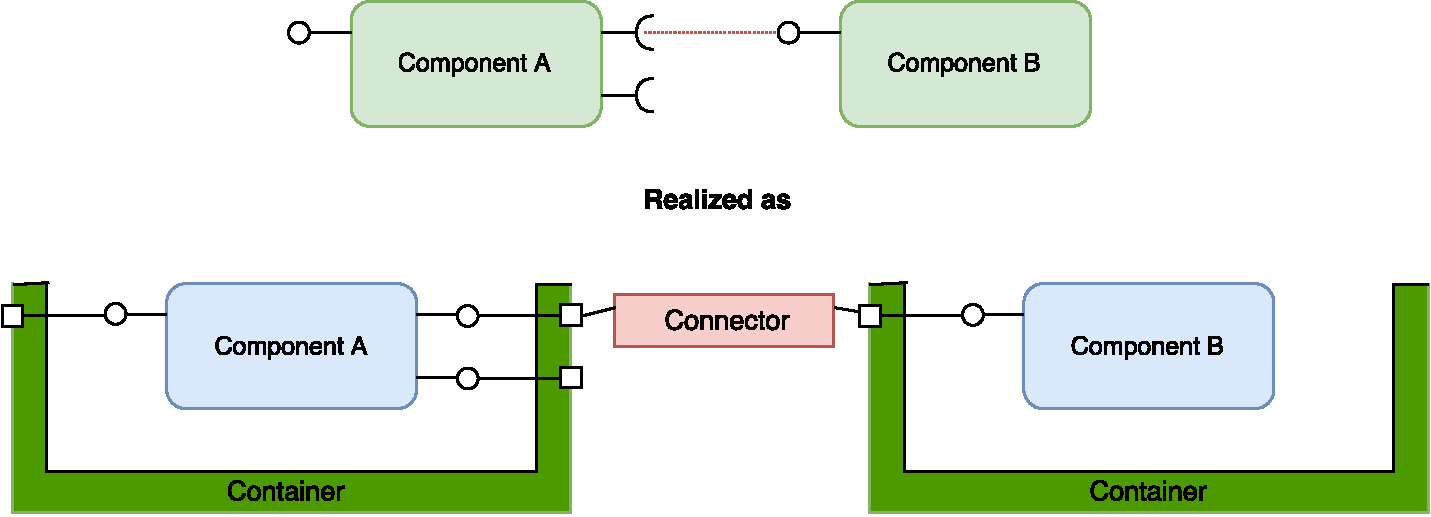
\includegraphics[width=0.8\textwidth]{ComponentContainerConnector.pdf}
	\caption{Components, containers and a connector connecting them}
	\source{\cite{SpecMetamodel}}
	\label{fig: Components containers and connectors}
\end{figure} 

\subsection{Computational model}
\label{section: Computational model} 
Using a computational model is necessary as per the Space Software engineering standard (ECSS-E-ST-440C) standard \cite{SAVOIR}. A dynamic software architecture is described according to an analyzable computational model which infers that the model development is fully consistent with that which underpins the mathematical equations which are used to predict the schedulability behavior of the system \cite{ScheduAnaly}. The computational model is more concerned about entities that belong to the implementation model (eg. tasks, protected objects and semaphores). A more abstract level description of these entities should be provided so that \cite{SAVOIR}:

\begin{itemize}
\item Pollution of the user-models with entities that are more primitive and are of interest to the lower levels of abstraction, is avoided. This is in line with the principle of separation of concerns, which is one of the high-level requirements.

\item The abstract representations represent the entities and their semantics faithfully.

\item Correct transformation of the information set by the designer in the higher-level representation to entities recognized by the computational model is ensured. This is in line with the principle of property preservation, which is also one of the high level requirements. 
\end{itemize} 

\subsection{Programming model and the execution platform}
\label{section: Execution platform}
The execution platform is a part of the software architecture providing all the necessary means for the implementation of a component and the computational model. It comprises of the middleware, the \ac{rtos}/\ac{rtk}, communication drivers and the \ac{bsp} for a given hardware platform. The services provided by the execution platform can be categorized into four different types \cite{SAVOIR}:

\begin{description}
\item [Services for containers] These services are meant to be used by the containers e.g. Tasking primitives, synchronization primitives, primitives related to time and timers.

\item [Services for connectors] These services are intended to be used by the connectors and it consists of actual communication means between components, ways to handle physical distribution across processing units, libraries used for translating data codes.

\item [Services to components] These services are supposed to be used by the components which implement the functional constraints. Typical services include: provision of on-board time for time-stamps, context management and data recovery. Access to these services are intercepted by the container wrapped around the component (refer \cref{section: Software entities}).

\item [Services to implement "abstract components"] These services include \ac{pus} monitoring, OBCPs, hardware representation etc.
\end{description}

It is important to note that different implementation of containers and connectors are necessary for each execution platform of interest.

The programming model realizes a given computational model and together with a conforming execution platform, it is possible to achieve the following goals \cite{PhdThesis}:

\begin{itemize}
\item Ensure that the implementation fully conforms with the semantics prescribed by the computational model and those assumed by the analysis.
\item Ensure that the contracts stipulated between the components are respected at run-time. This is in-line with the principle of property preservation which is one of the high level requirements.
\end{itemize} 

The achievement of those two goals would then warrant that the system represented for the analysis purposes is a faithful representation of its implementation and the results of the analysis performed on the system model would be a valid prediction of the system at run-time \cite{PhdThesis}.

The programming model, which is the subject of this Master thesis, is realized by adopting Tasking framework as a computational model whose concurrency semantics would conform to the analysis model.     
